\chapter{Fonctions du second degré}

La trajectoire d'un ballon, la forme d'une antenne parabolique ou l'aire d'un enclos : toutes ces situations se modélisent par une fonction du second degré.

Dans ce chapitre, on étudie les trois écritures d'un même trinôme, la résolution des équations et des inéquations associées, puis on les met au service de problèmes d'optimisation.

\section{Définition et différentes formes d'un trinôme}

\subsection{Forme développée}

\begin{df}
	On appelle \textbf{fonction polynôme du second degré} (ou \textbf{trinôme du second degré}) toute fonction $f$ définie sur $\R$ pouvant s'écrire sous la forme \textbf{développée} :
	\[
		f(x) = ax^2 + bx + c
	\]

	\ldots où $a$, $b$ et $c$ sont des nombres réels donnés, avec $a \neq 0$.
\end{df}

\begin{ex}
	\nline
	\begin{itemize}
		\item $f(x) = 2x^2 - 5x + 2$ est un trinôme du second degré, avec $a = 2$, $b = -5$ et $c = 2$.
		\item $g(x) = -x^2 + 4$ est un trinôme du second degré, avec $a = -1$, $b = 0$ et $c = 4$.
		\item $h(x) = (x-1)(3-2x)$ est un trinôme du second degré car en développant, on obtient :
		      \[
			      h(x) = -2x^2 + 5x - 3
		      \]

		      \ldots d'où $a = -2$, $b = 5$ et $c = -3$.
		\item $k(x) = (x+1)^2 - x^2$ n'est \emph{pas} un trinôme du second degré : en développant, on obtient $k(x) = 2x + 1$, qui est une fonction affine.
	\end{itemize}
\end{ex}

\begin{rem}
	La condition $a \neq 0$ est essentielle : si $a = 0$, la fonction $x \mapsto bx + c$ est affine.

	Par ailleurs, $f(0) = c$ : le nombre $c$ est l'ordonnée à l'origine de la courbe.
\end{rem}

\subsection{Forme canonique}

\begin{thm}
	Tout trinôme $f(x) = ax^2 + bx + c$ (avec $a \neq 0$) peut s'écrire, de manière unique, sous la forme \textbf{canonique} :
	\[
		f(x) = a(x - \alpha)^2 + \beta
		\qquad \text{avec} \qquad
		\alpha = \frac{-b}{2a} \quad \text{et} \quad \beta = f(\alpha)
	\]
\end{thm}

\newpage

\begin{demo}
	\nline
	\begin{itemize}
		\item \textbf{Existence.}

		      Comme $a \neq 0$, on factorise par $a$ :
		      \[
			      f(x) = a \left[ x^2 + \frac{b}{a}x + \frac{c}{a} \right]
		      \]

		      L'expression $x^2 + \dfrac{b}{a}x$ est le début du développement de $\left(x + \dfrac{b}{2a}\right)^2 = x^2 + \dfrac{b}{a}x + \dfrac{b^2}{4a^2}$.

		      Ainsi :
		      \[
			      x^2 + \frac{b}{a}x = \left(x + \frac{b}{2a}\right)^2 - \frac{b^2}{4a^2}
		      \]

		      En remplaçant dans l'expression de $f(x)$, il vient :
		      \[
			      f(x) = a \left[ \left(x + \frac{b}{2a}\right)^2 - \frac{b^2}{4a^2} + \frac{c}{a} \right]
			      = a \left[ \left(x + \frac{b}{2a}\right)^2 - \frac{b^2 - 4ac}{4a^2} \right]
		      \]

		      En distribuant le facteur $a$, on obtient :
		      \[
			      f(x) = a\left(x - \left(\frac{-b}{2a}\right)\right)^2 + \frac{4ac - b^2}{4a}
		      \]

		      On pose $\alpha = \dfrac{-b}{2a}$.

		      Pour $x = \alpha$, le terme $a(x-\alpha)^2$ s'annule, donc le dernier terme vaut bien $f(\alpha) = \beta$.

		\item \textbf{Unicité.}

		      Si $a(x-\alpha)^2 + \beta = a(x-\alpha')^2 + \beta'$ pour tout réel $x$, alors en développant et en identifiant les coefficients de $x$, on obtient $-2a\alpha = -2a\alpha'$, donc $\alpha = \alpha'$ car $a \neq 0$, puis $\beta = \beta'$.
	\end{itemize}
\end{demo}

\begin{methode}[Mettre un trinôme sous forme canonique]
	\nline
	\begin{enumerate}
		\item On identifie les coefficients $a$, $b$ et $c$.
		\item On calcule $\alpha = \dfrac{-b}{2a}$.
		\item On calcule $\beta = f(\alpha)$.
		\item On écrit $f(x) = a(x-\alpha)^2 + \beta$.
	\end{enumerate}
\end{methode}

\begin{ex}
	Soit $f(x) = 2x^2 - 8x + 3$.

	On a $a = 2$, $b = -8$ et $c = 3$, donc :
	\[
		\alpha = \frac{-\pa{-8}}{2 \times 2} = 2
		\qquad \text{et} \qquad
		\beta = f(2) = 2 \times 2^2 - 8 \times 2 + 3 = -5
	\]

	Ainsi $f(x) = 2(x-2)^2 - 5$.
\end{ex}

\begin{erreur}
	Dans la forme canonique, on écrit $(x - \alpha)^2$ :

	\begin{itemize}
		\item Si $\alpha = 2$, on écrit $(x-2)^2$ ;
		\item Si $\alpha = -3$, on écrit $(x+3)^2$.
	\end{itemize}

	Attention aussi au signe dans $\alpha = \dfrac{-b}{2a}$.
\end{erreur}

\subsection{Représentation graphique et variations}

La courbe représentative d'un trinôme du second degré est une \textbf{parabole}.

\begin{prop}
	Soit $f(x) = a(x-\alpha)^2 + \beta$ avec $a \neq 0$.
	\begin{itemize}
		\item La parabole possède un \textbf{sommet} $S\coordl{\alpha}{\beta}$.
		\item La droite d'équation $x = \alpha$ est un \textbf{axe de symétrie} de la parabole.
		\item Si $a > 0$, la parabole est \og tournée vers le haut\fg{} :
		      \begin{itemize}
			      \item $f$ est décroissante sur $\intof{-\infty}{\alpha}$, croissante sur $\intfo{\alpha}{+\infty}$,
			      \item $f$ admet un \textbf{minimum} égal à $\beta$, atteint en $x = \alpha$.
		      \end{itemize}
		\item Si $a < 0$, la parabole est \og tournée vers le bas\fg{} :

		      \begin{itemize}
			      \item $f$ est croissante sur $\intof{-\infty}{\alpha}$, décroissante sur $\intfo{\alpha}{+\infty}$,
			      \item et admet un \textbf{maximum} égal à $\beta$, atteint en $x = \alpha$.
		      \end{itemize}
	\end{itemize}
\end{prop}

\begin{center}
	\begin{minipage}[t]{0.48\linewidth}
		\centering
		\begin{tikzpicture}[scale=0.9]
			\draw[->] (-0.7,0) -- (3.9,0) node[right] {$x$};
			\draw[->] (0,-1.6) -- (0,2.8) node[above] {$y$};
			\draw[dashed, gris] (1.5,-1.4) -- (1.5,2.4) node[above] {\small $x=\alpha$};
			\draw[thick, bleu, domain=-0.2:3.2, samples=60, smooth] plot (\x, {0.8*(\x-1.5)^2-1});
			\draw[dashed, gris] (0,-1) -- (1.5,-1);
			\filldraw[rouge] (1.5,-1) circle (2pt) node[below right] {$S\coordl{\alpha}{\beta}$};
			\node[above right, rouge] at (1.5,0) {$\alpha$};
			\node[left, rouge] at (0,-1) {$\beta$};
		\end{tikzpicture}

		$a>0$ : minimum en $S$
	\end{minipage}\hfill
	\begin{minipage}[t]{0.48\linewidth}
		\centering
		\begin{tikzpicture}[scale=0.9]
			\draw[->] (-0.7,0) -- (3.9,0) node[right] {$x$};
			\draw[->] (0,-1.4) -- (0,2.4) node[above] {$y$};
			\draw[dashed, gris] (1.5,-1.2) node[below] {\small $x=\alpha$} -- (1.5,2.0);
			\draw[thick, bleu, domain=-0.2:3.2, samples=60, smooth] plot (\x, {-0.8*(\x-1.5)^2+1.5});
			\draw[dashed, gris] (0,1.5) -- (1.5,1.5);
			\filldraw[rouge] (1.5,1.5) circle (2pt) node[above right] {$S\coordl{\alpha}{\beta}$};
			\node[below right, rouge] at (1.5,0) {$\alpha$};
			\node[left, rouge] at (0,1.5) {$\beta$};
		\end{tikzpicture}

		$a<0$ : maximum en $S$
	\end{minipage}
\end{center}

\begin{prop}[Tableaux de variations]
	\nline
	\begin{center}
		\begin{minipage}[t]{0.48\linewidth}
			\centering
			$a>0$\par\ms
			\begin{tikzpicture}
				\tkzTabInit[lgt=1.5,espcl=2.2]{$x$/0.8,$f$/1.8}{$-\infty$,$\alpha$,$+\infty$}
				\tkzTabVar{+/$+\infty$,-/$\beta$,+/$+\infty$}
			\end{tikzpicture}
		\end{minipage}\hfill
		\begin{minipage}[t]{0.48\linewidth}
			\centering
			$a<0$\par\ms
			\begin{tikzpicture}
				\tkzTabInit[lgt=1.5,espcl=2.2]{$x$/0.8,$f$/1.8}{$-\infty$,$\alpha$,$+\infty$}
				\tkzTabVar{-/$-\infty$,+/$\beta$,-/$-\infty$}
			\end{tikzpicture}
		\end{minipage}
	\end{center}
\end{prop}

\begin{rem}
	Le coefficient $a$ commande aussi l'\og ouverture\fg{} de la parabole : plus $\abs{a}$ est grand, plus la parabole est resserrée autour de son axe de symétrie.

	\begin{center}
		\begin{minipage}[t]{0.48\linewidth}
			\centering
			\begin{tikzpicture}[>=Stealth]
				\begin{axis}[axis line style={thick}, width=\linewidth, height=5cm, axis lines=middle, xmin=-2.7, xmax=2.7, ymin=-0.5, ymax=5, xtick=\empty, ytick=\empty, legend columns=-1, legend style={at={(0.5,1.03)}, anchor=south}]
					\addplot[vert,  ultra thick, domain=-2.7:2.7, samples=60] {0.5*x^2};
					\addplot[dashed , bleu,  ultra thick, domain=-2.7:2.7, samples=60] {x^2};
					\addplot[dotted , rouge, ultra thick, domain=-2.7:2.7, samples=60] {2*x^2};
					\legend{$a=0.5\quad$, $a=1\quad$, $a=2$}
				\end{axis}
			\end{tikzpicture}
		\end{minipage}\hfill
		\begin{minipage}[t]{0.48\linewidth}
			\centering
			\begin{tikzpicture}[>=Stealth]
				\begin{axis}[axis line style={thick}, width=\linewidth, height=5cm, axis lines=middle, xmin=-2.7, xmax=2.7, ymin=-5, ymax=0.5, xtick=\empty, ytick=\empty, legend columns=-1, legend style={at={(0.5,1.03)}, anchor=south}]
					\addplot[vert,  ultra thick, domain=-2.7:2.7, samples=60] {-0.5*x^2};
					\addplot[dashed, bleu,  ultra thick, domain=-2.7:2.7, samples=60] {-x^2};
					\addplot[dotted, rouge, ultra thick, domain=-2.7:2.7, samples=60] {-2*x^2};
					\legend{$a=-0.5\quad$, $a=-1\quad$, $a=-2$}
				\end{axis}
			\end{tikzpicture}
		\end{minipage}
	\end{center}
\end{rem}

\section{Résolution d'équations du second degré}

\subsection{Discriminant et racines}

\begin{df}
	Soit $f(x) = ax^2 + bx + c$ un trinôme du second degré.
	\begin{itemize}
		\item On appelle \textbf{discriminant} de $f$ le nombre réel $\Delta = b^2 - 4ac$.
		\item On appelle \textbf{racine} de $f$ tout réel $x$ solution de l'équation $f(x) = 0$.
	\end{itemize}
\end{df}

\begin{thm}
	Le nombre de solutions réelles de l'équation $ax^2 + bx + c = 0$ (avec $a \neq 0$) dépend du signe de $\Delta$.
	\begin{itemize}
		\item Si $\Delta > 0$ : l'équation admet \textbf{deux solutions réelles distinctes}
		      \[
			      x_1 = \frac{-b - \sqrt{\Delta}}{2a} \qquad \text{et} \qquad x_2 = \frac{-b + \sqrt{\Delta}}{2a}
		      \]
		\item Si $\Delta = 0$ : l'équation admet \textbf{une unique solution}, appelée \textbf{racine double} :
		      \[
			      x_0 = \frac{-b}{2a}
		      \]
		\item Si $\Delta < 0$ : l'équation n'admet \textbf{aucune solution réelle}.
	\end{itemize}
\end{thm}

\begin{demo}
	D'après la démonstration précédente, pour tout réel $x$ :
	\[
		f(x) = a \left[ \left(x + \frac{b}{2a}\right)^2 - \frac{\Delta}{4a^2} \right]
	\]

	Comme $a \neq 0$, l'équation $f(x) = 0$ équivaut à :
	\[
		f(x) = 0 \iff \left(x + \dfrac{b}{2a}\right)^2 - \dfrac{\Delta}{4a^2}=0 \iff \left(x + \dfrac{b}{2a}\right)^2 = \dfrac{\Delta}{4a^2}
	\]

	Le dénominateur $4a^2 = (2a)^2$ est strictement positif : le membre de droite est donc du signe de $\Delta$.
	\begin{itemize}
		\item Si $\Delta > 0$, alors $\dfrac{\Delta}{4a^2} = \left(\dfrac{\sqrt{\Delta}}{2a}\right)^2$, et l'équation équivaut à $x + \dfrac{b}{2a} = \dfrac{\sqrt{\Delta}}{2a}$ ou $x + \dfrac{b}{2a} = \dfrac{-\sqrt{\Delta}}{2a}$, d'où $x_1$ et $x_2$.
		\item Si $\Delta = 0$, l'équation devient $\left(x + \dfrac{b}{2a}\right)^2 = 0$, d'où $x_0 = \dfrac{-b}{2a}$.
		\item Si $\Delta < 0$, le membre de droite est strictement négatif alors que le membre de gauche est un carré, donc positif ou nul : l'équation n'a pas de solution réelle.
	\end{itemize}
\end{demo}

\begin{rem}
	En comparant avec la forme canonique, on voit que $\beta = \dfrac{-\Delta}{4a}$, soit $\Delta = -4a\beta$.

	Le nombre de racines traduit donc la position du sommet par rapport à l'axe des abscisses.

	Par exemple, pour $a > 0$, le sommet est sous l'axe ($\beta < 0$) exactement quand $\Delta > 0$.
\end{rem}

\newpage

\begin{prop}[Position de la parabole selon $a$ et $\Delta$]
	\nc{\parabolecas}[2]{%
		\draw[->] (-0.3,0) -- (4.5,0) node[right] {$x$};
		\draw[->] (0,-1.7) -- (0,2.4) node[above] {$y$};
		\begin{scope}
			\clip (0.01,-1.6) rectangle (4.2,2.2);
			\draw[thick, bleu, domain=0:4, samples=60, smooth] plot (\x, {#1*(\x-2)^2+(#2)});
		\end{scope}
	}
	\nline
	\begin{center}
		\begin{minipage}[t]{0.32\linewidth}
			\centering
			\begin{tikzpicture}[scale=0.8]
				\parabolecas{0.5}{-1}
				\filldraw[rouge] (0.586,0) circle (2pt) (3.414,0) circle (2pt);
				\node[above right, rouge] at (0.586,0) {$x_1$};
				\node[above left, rouge] at (3.414,0) {$x_2$};
			\end{tikzpicture}

			$a>0$ et $\Delta>0$
		\end{minipage}\hfill
		\begin{minipage}[t]{0.32\linewidth}
			\centering
			\begin{tikzpicture}[scale=0.8]
				\parabolecas{0.5}{0}
				\filldraw[rouge] (2,0) circle (2pt);
				\node[below, rouge] at (2,0) {$x_0$};
			\end{tikzpicture}

			$a>0$ et $\Delta=0$
		\end{minipage}\hfill
		\begin{minipage}[t]{0.32\linewidth}
			\centering
			\begin{tikzpicture}[scale=0.8]
				\parabolecas{0.5}{1}
			\end{tikzpicture}

			$a>0$ et $\Delta<0$
		\end{minipage}

		\bigskip

		\begin{minipage}[t]{0.32\linewidth}
			\centering
			\begin{tikzpicture}[scale=0.8]
				\parabolecas{-0.5}{1}
				\filldraw[rouge] (0.586,0) circle (2pt) (3.414,0) circle (2pt);
				\node[below right, rouge] at (0.586,0) {$x_1$};
				\node[below left, rouge] at (3.414,0) {$x_2$};
			\end{tikzpicture}

			$a<0$ et $\Delta>0$
		\end{minipage}\hfill
		\begin{minipage}[t]{0.32\linewidth}
			\centering
			\begin{tikzpicture}[scale=0.8]
				\parabolecas{-0.5}{0}
				\filldraw[rouge] (2,0) circle (2pt);
				\node[above, rouge] at (2,0) {$x_0$};
			\end{tikzpicture}

			$a<0$ et $\Delta=0$
		\end{minipage}\hfill
		\begin{minipage}[t]{0.32\linewidth}
			\centering
			\begin{tikzpicture}[scale=0.8]
				\parabolecas{-0.5}{-1}
			\end{tikzpicture}

			$a<0$ et $\Delta<0$
		\end{minipage}
	\end{center}
\end{prop}

\begin{methode}[Résoudre une équation du second degré]
	\nline
	\begin{enumerate}
		\item On identifie $a$, $b$ et $c$.
		\item On calcule le discriminant $\Delta = b^2 - 4ac$.
		\item On conclut selon le signe de $\Delta$ (deux solutions, une solution ou aucune), en utilisant les formules du théorème.
		\item On écrit l'ensemble $S$ des solutions.
	\end{enumerate}
\end{methode}

\begin{ex}
	Résoudre dans $\R$ les équations suivantes.
	\begin{enumerate}
		\item $2x^2 - 5x + 2 = 0$. Ici $a = 2$, $b = -5$, $c = 2$, donc :
		      \[
			      \Delta = b^2-4ac = (-5)^2 - 4 \times 2 \times 2 = 25 - 16 = 9 > 0
		      \]

		      L'équation a deux solutions :
		      \[
			      x_1 = \frac{5 - \sqrt{9}}{2 \times 2} = \frac{1}{2}
			      \qquad \text{et} \qquad
			      x_2 = \frac{5 + \sqrt{9}}{2 \times 2} = 2,
			      \qquad \text{donc} \qquad
			      S = \brac{\frac{1}{2}\,;\,2}
		      \]
		\item $x^2 - 6x + 9 = 0$.

		      Ici $\Delta = (-6)^2 - 4 \times 1 \times 9 = 0$, donc l'équation a une unique solution $x_0 = \dfrac{6}{2} = 3$, et $S = \brac{3}$.

		\item $x^2 + x + 1 = 0$.

		      Ici $\Delta = 1^2 - 4 \times 1 \times 1 = -3 < 0$, donc $S = \varnothing$.

	\end{enumerate}
\end{ex}

\begin{piege}
	Lors du calcul de $b^2$ avec $b$ négatif, les parenthèses sont indispensables : si $b = -5$, alors $b^2 = (-5)^2 = 25$ et non $-5^2 = -25$.
\end{piege}

\begin{attention}
	Dans les formules des racines, la barre de fraction porte sur \emph{tout} le numérateur $-b \pm \sqrt{\Delta}$, et le dénominateur est $2a$ (et pas seulement $2$).
\end{attention}

\begin{rem}
	Dans deux cas particuliers, le discriminant est inutile.
	\begin{itemize}
		\item Si $c = 0$ : $ax^2 + bx = x(ax + b) = 0$, donc $x = 0$ ou $x = \dfrac{-b}{a}$.
		\item Si $b = 0$ : $ax^2 + c = 0$ équivaut à $x^2 = \dfrac{-c}{a}$, qui admet des solutions réelles uniquement si $\dfrac{-c}{a} \geq 0$.

		      Dans ce cas, on a :
		      \[
			      x_1=\sqrt{\dfrac{-c}{a}}\qquad\text{et}\qquad x_2=-\sqrt{\dfrac{-c}{a}}
		      \]
	\end{itemize}
\end{rem}

\subsection{Forme factorisée}

\begin{prop}
	Soit $f(x) = ax^2 + bx + c$ un trinôme du second degré.
	\begin{itemize}
		\item Si $\Delta > 0$ : $f(x) = a(x - x_1)(x - x_2)$, où $x_1$ et $x_2$ sont les deux racines.
		\item Si $\Delta = 0$ : $f(x) = a(x - x_0)^2$, où $x_0$ est la racine double.
		\item Si $\Delta < 0$ : $f$ ne se factorise pas dans $\R$.
	\end{itemize}
\end{prop}

\begin{demo}
	\nline
	\begin{itemize}
		\item Si $\Delta > 0$, on utilise l'identité $A^2 - B^2 = (A-B)(A+B)$ dans la forme canonique :
		      \[
			      f(x) = a \left[ \left(x + \frac{b}{2a}\right)^2 - \left(\frac{\sqrt{\Delta}}{2a}\right)^2 \right]
			      = a \left( x + \frac{b}{2a} - \frac{\sqrt{\Delta}}{2a} \right)\left( x + \frac{b}{2a} + \frac{\sqrt{\Delta}}{2a} \right)
			      = a(x - x_2)(x - x_1)
		      \]

		\item Si $\Delta = 0$, la forme canonique est directement :
		      \[
			      f(x) = a\left(x + \dfrac{b}{2a}\right)^2 = a(x - x_0)^2
		      \]

		\item Si $\Delta < 0$, la forme canonique $a\left[\left(x + \dfrac{b}{2a}\right)^2 + \dfrac{-\Delta}{4a^2}\right]$ ne s'annule jamais : $f$ n'a pas de racine, donc aucune factorisation de la forme $a(x - r)(\cdots)$ n'existe.
	\end{itemize}
\end{demo}

\begin{ex}
	Pour $f(x) = 2x^2 - 5x + 2$, les racines sont $\dfrac{1}{2}$ et $2$, donc
	\[
		f(x) = 2\left(x - \frac{1}{2}\right)(x - 2) = (2x - 1)(x - 2)
	\]
\end{ex}

\subsection{Somme et produit des racines}

\begin{prop}
	Si le trinôme $f(x) = ax^2 + bx + c$ possède deux racines $x_1$ et $x_2$ (distinctes ou confondues), alors
	\[
		x_1 + x_2 = \frac{-b}{a} \qquad \text{et} \qquad x_1 \times x_2 = \frac{c}{a}
	\]
\end{prop}

\begin{demo}
	D'après la forme factorisée,
	\[
		ax^2 + bx + c = a(x - x_1)(x - x_2) = ax^2 - a(x_1 + x_2)x + a\,x_1 x_2
	\]

	Par identification des coefficients : $b = -a(x_1 + x_2)$ et $c = a\,x_1 x_2$, d'où le résultat.
\end{demo}

\begin{methode}[Trouver deux nombres connaissant leur somme et leur produit]
	Deux nombres de somme $S$ et de produit $P$ sont les solutions (si elles existent) de l'équation :
	\[
		x^2 - Sx + P = 0
	\]
\end{methode}

\begin{ex}
	On cherche deux nombres de somme $7$ et de produit $12$.

	Ce sont les solutions de $x^2 - 7x + 12 = 0$.

	On a $\Delta = 49 - 48 = 1$, donc :
	\[
		x_1 = \dfrac{7 - 1}{2} = 3\qquad\text{et}\qquad x_2 = \dfrac{7 + 1}{2} = 4
	\]

\end{ex}

\begin{prop}[Racines évidentes]
	Soit $f(x) = ax^2 + bx + c$ avec $a \neq 0$.
	\begin{itemize}
		\item Si $a + b + c = 0$, alors $1$ est racine et l'autre racine est $\dfrac{c}{a}$.
		\item Si $a - b + c = 0$, alors $-1$ est racine et l'autre racine est $\dfrac{-c}{a}$.
	\end{itemize}
\end{prop}

\begin{demo}
	Soit $f(x) = ax^2 + bx + c$ avec $a \neq 0$.
	\begin{itemize}
		\item Si $a + b + c = 0$, alors $f(1) = a+b+c = 0$.

		      Le produit des racines valant $\dfrac{c}{a}$, l'autre racine est $\dfrac{c}{a}$.

		\item Si $a - b + c = 0$, alors $f(-1) = 0$ et l'autre racine $r$ vérifie $-r = \dfrac{c}{a}$.
	\end{itemize}
\end{demo}

\begin{ex}
	Pour $3x^2 - 5x + 2$, on a $3 - 5 + 2 = 0$ donc les racines sont $1$ et $\dfrac{2}{3}$.
\end{ex}

\section{Signe d'un trinôme et inéquations}

\subsection{Signe d'un trinôme}

\begin{thm}
	Soit $f(x) = ax^2 + bx + c$ avec $a \neq 0$.
	\begin{itemize}
		\item Si $\Delta > 0$ : $f(x)$ est du \textbf{signe de $a$ à l'extérieur des racines} et du \textbf{signe opposé à celui de $a$ entre les racines}.
		\item Si $\Delta = 0$ : $f(x)$ est du signe de $a$ pour tout $x \neq x_0$, et s'annule en $x_0$.
		\item Si $\Delta < 0$ : $f(x)$ est strictement du signe de $a$ pour tout réel $x$.
	\end{itemize}
\end{thm}

\begin{demo}
	\nline
	\begin{itemize}
		\item Si $\Delta > 0$, on a $f(x) = a(x - x_1)(x - x_2)$ avec $x_1 < x_2$.

		      Le produit $(x - x_1)(x - x_2)$ est :
		      \begin{itemize}
			      \item strictement positif si $x < x_1 < x_2$ ou $x_1 < x_2 < x$,
			      \item et strictement négatif si $x_1 < x < x_2$.
		      \end{itemize}
		\item Si $\Delta = 0$, $f(x) = a(x - x_0)^2$ et $(x - x_0)^2 > 0$ pour $x \neq x_0$.
		\item Si $\Delta < 0$, $f(x) = a\left[\left(x + \dfrac{b}{2a}\right)^2 + \dfrac{-\Delta}{4a^2}\right]$ et le crochet est strictement positif.
	\end{itemize}
\end{demo}

\newpage

\begin{prop}[Tableaux de signes]
	On note $x_1 < x_2$ les racines lorsqu'elles existent.
	\begin{center}
		\renewcommand{\arraystretch}{1.6}
		\begin{tabular}{@{}m{1.4cm}@{}m{7.5cm}@{}m{7.5cm}@{}}
			           & \centering $a>0$ & \centering\arraybackslash $a<0$ \\
			$\Delta>0$ &
			\centering
			\begin{tikzpicture}
				\tkzTabInit[lgt=1.4,espcl=1.3]{$x$/0.8,$f(x)$/0.8}{$-\infty$,$x_1$,$x_2$,$+\infty$}
				\tkzTabLine{,+,z,-,z,+,}
			\end{tikzpicture}
			           &
			\centering\arraybackslash
			\begin{tikzpicture}
				\tkzTabInit[lgt=1.4,espcl=1.3]{$x$/0.8,$f(x)$/0.8}{$-\infty$,$x_1$,$x_2$,$+\infty$}
				\tkzTabLine{,-,z,+,z,-,}
			\end{tikzpicture}
			\\
			$\Delta=0$ &
			\centering
			\begin{tikzpicture}
				\tkzTabInit[lgt=1.4,espcl=1.95]{$x$/0.8,$f(x)$/0.8}{$-\infty$,$x_0$,$+\infty$}
				\tkzTabLine{,+,z,+,}
			\end{tikzpicture}
			           &
			\centering\arraybackslash
			\begin{tikzpicture}
				\tkzTabInit[lgt=1.4,espcl=1.95]{$x$/0.8,$f(x)$/0.8}{$-\infty$,$x_0$,$+\infty$}
				\tkzTabLine{,-,z,-,}
			\end{tikzpicture}
			\\
			$\Delta<0$ &
			\centering
			\begin{tikzpicture}
				\tkzTabInit[lgt=1.4,espcl=3.9]{$x$/0.8,$f(x)$/0.8}{$-\infty$,$+\infty$}
				\tkzTabLine{,+,}
			\end{tikzpicture}
			           &
			\centering\arraybackslash
			\begin{tikzpicture}
				\tkzTabInit[lgt=1.4,espcl=3.9]{$x$/0.8,$f(x)$/0.8}{$-\infty$,$+\infty$}
				\tkzTabLine{,-,}
			\end{tikzpicture}
		\end{tabular}
	\end{center}
\end{prop}

\subsection{Résolution d'inéquations du second degré}

\begin{methode}[Résoudre une inéquation du second degré]
	\nline
	\begin{enumerate}
		\item On se ramène à une inéquation du type $f(x) \geq 0$, $f(x) > 0$, $f(x) \leq 0$ ou $f(x) < 0$.
		\item On calcule $\Delta$ et, s'il y en a, les racines de $f$.
		\item On dresse le tableau de signes de $f$ en tenant compte du signe de $a$.
		\item On lit les intervalles solutions : les racines sont incluses si l'inégalité est large ($\geq$ ou $\leq$), exclues si elle est stricte.
	\end{enumerate}
\end{methode}

\begin{ex}
	Résoudre $x^2 - x - 6 \geq 0$.

	On a $\Delta = (-1)^2 - 4 \times 1 \times (-6) = 25 > 0$, donc les racines sont $x_1 = \dfrac{1 - 5}{2} = -2$ et $x_2 = \dfrac{1 + 5}{2} = 3$.

	Comme $a = 1 > 0$, on obtient :
	\begin{center}
		\begin{tikzpicture}
			\tkzTabInit[lgt=3,espcl=2]{$x$/0.8,$x^2-x-6$/0.8}{$-\infty$,$-2$,$3$,$+\infty$}
			\tkzTabLine{,+,z,-,z,+,}
		\end{tikzpicture}
	\end{center}

	L'inégalité est large, donc on garde les racines :
	\[
		S = \intof{-\infty}{-2} \cup \intfo{3}{+\infty}
	\]
	\begin{center}
		\begin{tikzpicture}[x=0.8cm, y=0.33cm]
			\draw[->] (-4.4,0) -- (4.9,0) node[right] {$x$};
			\draw[->] (0,-7) -- (0,8.3) node[above] {$y$};
			\draw[thick, bleu, domain=-3.2:4.2, samples=80, smooth] plot (\x, {\x*\x-\x-6});
			\draw[very thick, rouge, domain=-3.2:-2, samples=30] plot (\x, {\x*\x-\x-6});
			\draw[very thick, rouge, domain=3:4.2, samples=30] plot (\x, {\x*\x-\x-6});
			\draw[line width=2pt, rouge] (-4.2,0) -- (-2,0);
			\draw[line width=2pt, rouge] (3,0) -- (4.7,0);
			\filldraw[rouge] (-2,0) circle (2pt) (3,0) circle (2pt);
			\node[below left, rouge] at (-2,0) {$-2$};
			\node[below right, rouge] at (3,0) {$3$};
		\end{tikzpicture}
	\end{center}
	Les solutions sont les abscisses des points de la parabole situés sur ou au-dessus de l'axe des abscisses.
\end{ex}

\begin{ex}
	Résoudre $-2x^2 + 3x + 2 > 0$.

	On a $\Delta = 3^2 - 4 \times (-2) \times 2 = 25 > 0$, donc les racines sont $\dfrac{-3 - 5}{-4} = 2$ et $\dfrac{-3 + 5}{-4} = \dfrac{-1}{2}$.

	Comme $a = -2 < 0$ :
	\begin{center}
		\begin{tikzpicture}
			\tkzTabInit[lgt=3.4,espcl=2]{$x$/0.8,$-2x^2+3x+2$/0.8}{$-\infty$,$\frac{-1}{2}$,$2$,$+\infty$}
			\tkzTabLine{,-,z,+,z,-,}
		\end{tikzpicture}
	\end{center}

	L'inégalité est stricte, donc $S = \intoo{\frac{-1}{2}}{2}$.
\end{ex}

\begin{ex}
	Résoudre $x^2 + 2x + 3 < 0$.

	On a $\Delta = 4 - 12 = -8 < 0$ et $a = 1 > 0$ : le trinôme est strictement positif sur $\R$, donc $S = \varnothing$.
\end{ex}

\section{Synthèse et problèmes d'optimisation}

\subsection{Choisir la forme adaptée}

\begin{center}
	\renewcommand{\arraystretch}{1.5}
	\begin{tabular}{|>{\raggedright\arraybackslash}m{3.6cm}|>{\centering\arraybackslash}m{4.4cm}|>{\raggedright\arraybackslash}m{7.6cm}|}
		\hline
		\ccg \textbf{Forme}                      & \ccg \textbf{Expression}  & \ccg \textbf{Utilisation privilégiée}                                            \\ \hline
		\textbf{Développée}                      & $ax^2 + bx + c$           & Lire $a$, $b$, $c$ ; calculer $\Delta$ ; lire l'ordonnée à l'origine $f(0) = c$. \\ \hline
		\textbf{Canonique}                       & $a(x - \alpha)^2 + \beta$ & Déterminer le sommet $S\coordl{\alpha}{\beta}$, les variations et l'extremum.    \\ \hline
		\textbf{Factorisée} (si $\Delta \geq 0$) & $a(x - x_1)(x - x_2)$     & Résoudre $f(x) = 0$ ; étudier le signe de $f(x)$.                                \\ \hline
	\end{tabular}
\end{center}

\subsection{Problèmes d'optimisation}

\begin{methode}[Résoudre un problème d'optimisation]
	\nline
	\begin{enumerate}
		\item On choisit une variable $x$ et on précise l'ensemble de valeurs possibles.
		\item On exprime la grandeur à optimiser sous la forme d'un trinôme $f(x)$.
		\item On détermine la forme canonique de $f$, donc son sommet $S\coordl{\alpha}{\beta}$.
		\item Selon le signe de $a$, on conclut :

		      $\beta$ est le maximum ($a < 0$) ou le minimum ($a > 0$), atteint pour $x = \alpha$, à condition que $\alpha$ appartienne à l'ensemble de valeurs possibles.
	\end{enumerate}
\end{methode}

\begin{ex}
	Un agriculteur dispose de $40\,\text{m}$ de clôture pour former un enclos rectangulaire.

	Quelle largeur choisir pour que l'aire de l'enclos soit maximale ?

	\bigskip

	\begin{minipage}[c]{0.36\linewidth}
		\centering
		\begin{tikzpicture}
			\draw[thick, bleu, fill=bleu!10] (0,0) rectangle (3.6,1.8);
			\draw[<->] (0,-0.3) -- (3.6,-0.3) node[midway, below] {$20-x$};
			\draw[<->] (3.9,0) -- (3.9,1.8) node[midway, right] {$x$};
		\end{tikzpicture}
	\end{minipage}\hfill
	\begin{minipage}[c]{0.60\linewidth}
		\begin{tikzpicture}
			\begin{axis}[axis line style={thick}, width=\linewidth, height=5.4cm, axis lines=left,
					xmin=0, xmax=21, ymin=0, ymax=125, xtick={0,10,20}, ytick={0,50,100},
					xlabel={$x$}, ylabel={$A(x)$}]
				\addplot[bleu, thick, domain=0:20, samples=60] {-x^2+20*x};
				\draw[dashed, rouge] (axis cs:10,0) -- (axis cs:10,100) -- (axis cs:0,100);
				\filldraw[rouge] (axis cs:10,100) circle (2pt);
				\node[above right, rouge] at (axis cs:10,100) {$M\coordl{10}{100}$};
			\end{axis}
		\end{tikzpicture}
	\end{minipage}

	\medskip
	\begin{enumerate}
		\item \textbf{Expression de l'aire.}

		      Le demi-périmètre vaut $20\,\text{m}$ : si la largeur est $x$, la longueur est $20 - x$, avec $x \in \intff{0}{20}$.

		      L'aire est :
		      \[
			      A(x) = x(20 - x) = -x^2 + 20x
		      \]

		\item \textbf{Forme canonique.}

		      Ici $a = -1$, $b = 20$, $c = 0$, donc :
		      \[
			      \alpha = \frac{-20}{2 \times (-1)} = 10
			      \qquad \text{et} \qquad
			      \beta = A(10) = -100 + 200 = 100
		      \]

		      \ldots d'où $A(x) = -(x - 10)^2 + 100$.

		\item \textbf{Conclusion.}

		      Comme $a = -1 < 0$ et $10 \in \intff{0}{20}$, donc $A(x)$ admet un maximum égal à $100\,\text{m}^2$, atteint pour $x = 10\,\text{m}$.

		      L'enclos d'aire maximale est alors un carré de côté $10\,\text{m}$.
	\end{enumerate}
\end{ex}

